\documentclass[tikz,border=8pt]{standalone}
% Shared look for every TikZ diagram. Load with \input{../../tools/tikz-style.tex}
\usepackage[sfdefault]{roboto}
\usetikzlibrary{arrows.meta, positioning, shapes.geometric, calc, fit, backgrounds}
\definecolor{cblue}{HTML}{4C78A8}
\definecolor{corange}{HTML}{F58518}
\definecolor{cgreen}{HTML}{54A24B}
\definecolor{cred}{HTML}{E45756}
\definecolor{cpurple}{HTML}{B279A2}
\definecolor{cgrey}{HTML}{6B6B6B}
\tikzset{
  every picture/.style={font=\sffamily, line width=1.2pt},
  box/.style={draw=#1, fill=#1!12, rounded corners=4pt, align=center, inner sep=7pt, minimum height=1.1cm},
  box/.default=cgrey,
  arrow/.style={-{Stealth[length=3mm]}, draw=cgrey, line width=1.4pt},
  title/.style={font=\sffamily\bfseries\Large},
  note/.style={font=\sffamily\small, text=cgrey, align=center},
}
\AtBeginDocument{\hyphenpenalty=10000 \exhyphenpenalty=10000}

% Distance between two headings on a dial. Left: 350 and 15 degrees; plain subtraction gives the long way, 335
% degrees; the angular distance takes the short way across 0, 25 degrees. Right: the triangle inequality on the
% dial: 350 -> 0 -> 15 is 10 + 15 = 25 degrees, no shorter than going straight, 25 degrees.
\begin{document}
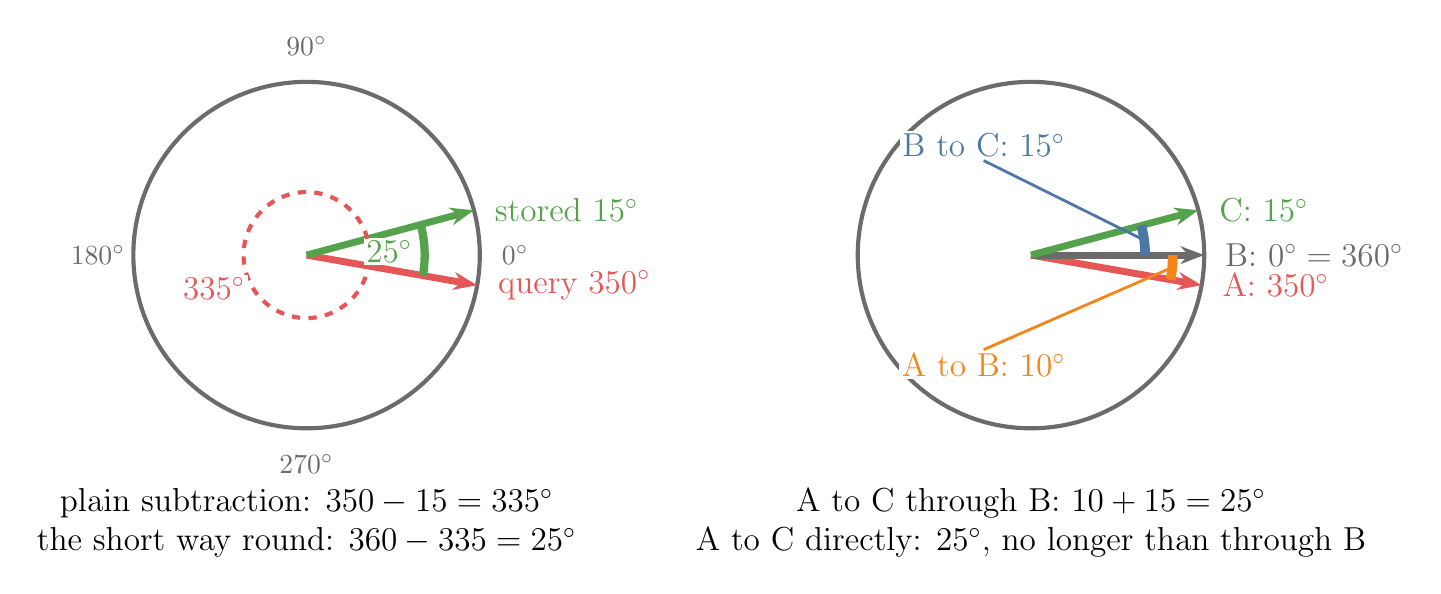
\begin{tikzpicture}[every node/.append style={font=\large}]
  \begin{scope}
    \draw[cgrey, line width=1.5pt] (0,0) circle (2.2);
    \foreach \a/\l in {0/0^\circ, 90/90^\circ, 180/180^\circ, 270/270^\circ}
      \node[cgrey, font=\normalsize] at (\a:2.65) {$\l$};
    \draw[cred, line width=2.5pt, -{Stealth[length=3mm]}] (0,0) -- (350:2.2) node[right=3pt] {query $350^\circ$};
    \draw[cgreen, line width=2.5pt, -{Stealth[length=3mm]}] (0,0) -- (15:2.2) node[right=3pt] {stored $15^\circ$};
    \draw[cgreen, line width=3pt] (350:1.5) arc[start angle=-10, end angle=15, radius=1.5];
    \node[cgreen, fill=white, inner sep=1pt] at (2.5:1.05) {$25^\circ$};
    \draw[cred, dashed, line width=1.5pt] (15:0.8) arc[start angle=15, end angle=350, radius=0.8];
    \node[cred, fill=white, inner sep=1pt] at (200:1.25) {$335^\circ$};
    \node[align=center] at (0,-3.4) {plain subtraction: $350 - 15 = 335^\circ$\\ the short way round: $360 - 335 = 25^\circ$};
  \end{scope}
  \begin{scope}[xshift=9.2cm]
    \draw[cgrey, line width=1.5pt] (0,0) circle (2.2);
    \draw[cred, line width=2.5pt, -{Stealth[length=3mm]}] (0,0) -- (350:2.2) node[right=3pt] {A: $350^\circ$};
    \draw[cgrey, line width=2.5pt, -{Stealth[length=3mm]}] (0,0) -- (0:2.2) node[right=3pt] {B: $0^\circ = 360^\circ$};
    \draw[cgreen, line width=2.5pt, -{Stealth[length=3mm]}] (0,0) -- (15:2.2) node[right=3pt] {C: $15^\circ$};
    \draw[corange, line width=3.5pt] (350:1.8) arc[start angle=-10, end angle=0, radius=1.8];
    \draw[cblue, line width=3.5pt] (0:1.45) arc[start angle=0, end angle=15, radius=1.45];
    \draw[corange, line width=1pt] (355:1.8) -- (-0.6,-1.2) node[below, fill=white, inner sep=1pt] {A to B: $10^\circ$};
    \draw[cblue, line width=1pt] (7.5:1.45) -- (-0.6,1.2) node[above, fill=white, inner sep=1pt] {B to C: $15^\circ$};
    \node[align=center] at (0,-3.4) {A to C through B: $10 + 15 = 25^\circ$\\ A to C directly: $25^\circ$, no longer than through B};
  \end{scope}
\end{tikzpicture}
\end{document}
